\section{Data}
\label{sec:data}

\subsection{Sources}

The panel combines four kinds of source, each archived as raw files with the source URL,
retrieval time and HTTP status. (1) AWS's public price-list offer files, which give on-demand and
reserved list prices roughly monthly since 2015. (2) The SkyPilot project's public catalog history,
which records AWS, Azure, Google Cloud and Lambda list and spot prices since mid-2022. SkyPilot's
catalog carries no licence, so it is used but not redistributed. (3) Archived pricing pages for
Lambda, CoreWeave and Paperspace from the Internet Archive's Wayback Machine. (4) Live daily
collection from October 2026 (the Azure Retail Prices API, AWS offer files, Lambda's pricing page
and SkyPilot). Chip specifications and release dates come from Epoch AI's hardware database
\citep{epoch2026hardware}, electricity prices from the U.S. Energy Information Administration,
and the deflator is the BLS CPI-U \citep{blscpiu}. Vast.ai, RunPod and Oracle restrict automated
collection, so nothing is collected from them.

\subsection{Construction}

The unit of observation is one posted price for a provider, SKU, chip, GPU count, interconnect,
region, contract type and term in one month, in U.S. dollars per GPU-hour; multi-GPU instance
prices are divided by the GPU count. From \nRawRows{} raw rows, zone-level spot prices become one
regional median per day, daily observations become one monthly median, and where two collectors
record the same offer in the same month the more direct source is kept (the two agree to a median
gap of zero). The result is \nPanelRows{} listing-months from October 2017 to November 2026. Real
prices are in 2025 dollars. The estimation sample drops the L40S (no release date), the MI300X (one
month), outlier-flagged prices and the partial month of November 2026, leaving \nSampleRows{}
listing-months for seven NVIDIA chips (Table~\ref{tab:sample}).

\begin{table}[htbp]
\centering
\caption{Estimation sample by chip}
\label{tab:sample}
\begin{adjustbox}{max width=\textwidth}
% Generated by gel.viz.paper_numbers from p4_descriptive_facts.csv and p5_sample.csv.
\begin{tabular}{lrrrrrr}
\hline
Chip & Listing-months & Providers & First month & Ages (months) & Hyperscaler/neocloud & Max/min provider \\
\hline
V100 & 5{,}260 & 6 & 2017-10 & 3--111 & 1.61 & 3.10 \\
A100 40GB & 5{,}510 & 6 & 2020-11 & 6--77 & 2.34 & 2.67 \\
A100 80GB & 3{,}081 & 6 & 2022-05 & 18--71 & 1.92 & 2.47 \\
H100 PCIe & 355 & 3 & 2023-01 & 4--49 & 2.66 & 1.95 \\
H100 SXM & 4{,}831 & 6 & 2023-01 & 4--49 & 3.10 & 3.52 \\
H200 & 664 & 4 & 2024-12 & 1--23 & 0.73 & 1.73 \\
B200 & 484 & 4 & 2025-06 & 7--23 & 1.54 & 2.08 \\
\hline
\end{tabular}

\end{adjustbox}
\par\smallskip\footnotesize Listing-months in the estimation sample; ages in months since the
Epoch release month. ``Hyperscaler/neocloud'' is the median ratio of median on-demand prices in
months where both provider types list the chip; ``Max/min provider'' is the median ratio of the
most to the least expensive provider's median on-demand price.
\end{table}

\subsection{What the raw panel shows}

The panel is mostly hyperscaler list prices: hyperscalers account for \nHyperscalerShare{} of
listing-months and Google Cloud alone for \nGoogleShare{} of the estimation sample, because it
publishes every region and machine shape. Neocloud history (\nNeocloudRows{} listing-months)
comes from archived pages. Three features of the raw data matter for everything that follows.

\emph{Prices barely move.} \nListUnchanged{} of the \nListTransitions{} month-to-month transitions
in on-demand and reserved listings show no price change; AWS spot prices, by contrast, are
unchanged in only \nAwsSpotUnchanged{} of transitions.

\emph{Levels differ widely across providers.} For the H100 SXM the median hyperscaler on-demand
price is \nHHundredHypNeo{} times the neocloud price, and the most expensive provider's median is
\nHHundredDispersion{} times the cheapest's in a typical month (Table~\ref{tab:sample},
Figure~\ref{fig:prices}).

\emph{Raw prices rise with age for the newest chips} (Figure~\ref{fig:prices}, right), because age
moves one-for-one with calendar time, with the 2023--26 shortages and with which providers list a
chip. \ajcheck{None of this is an age effect, which is why the paper does not read age profiles off
raw prices.}

\begin{figure}[htbp]
\centering
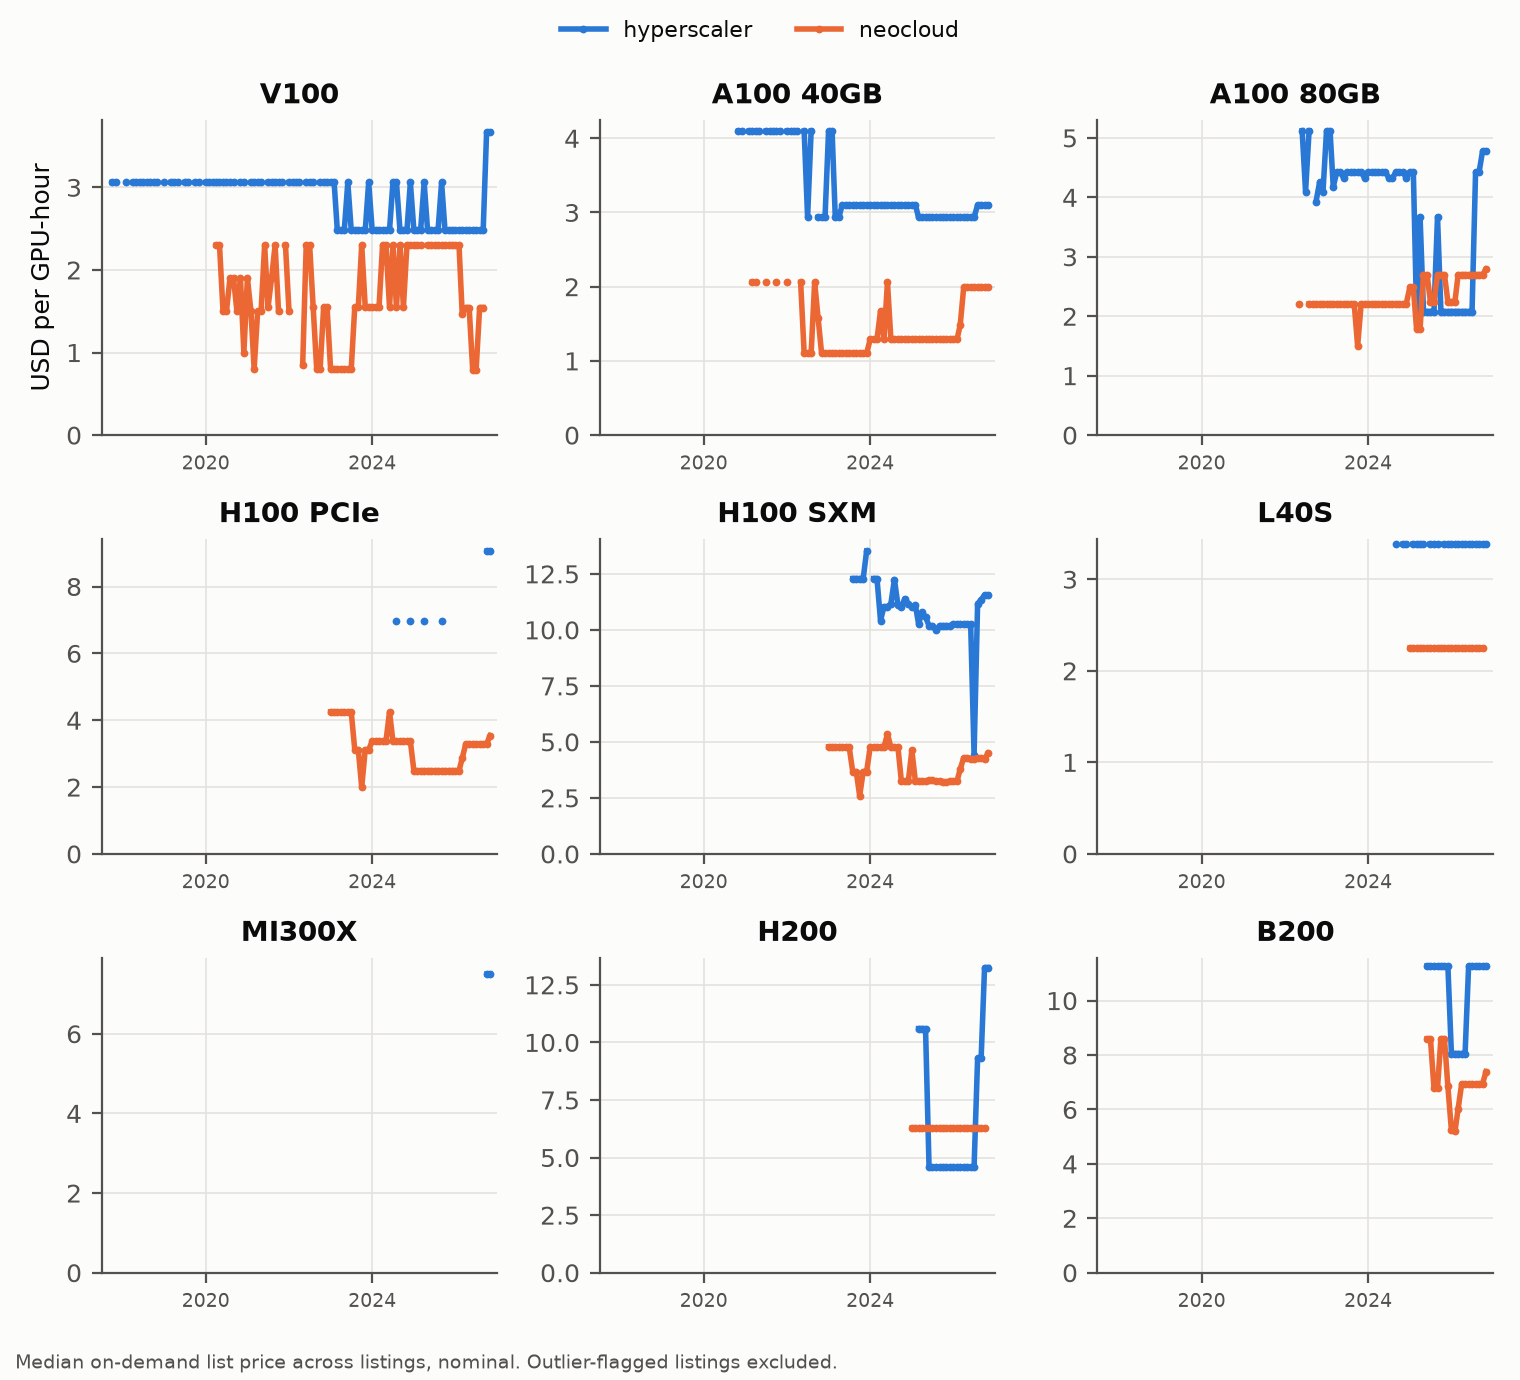
\includegraphics[width=0.49\textwidth]{p4a_price_by_chip.png}
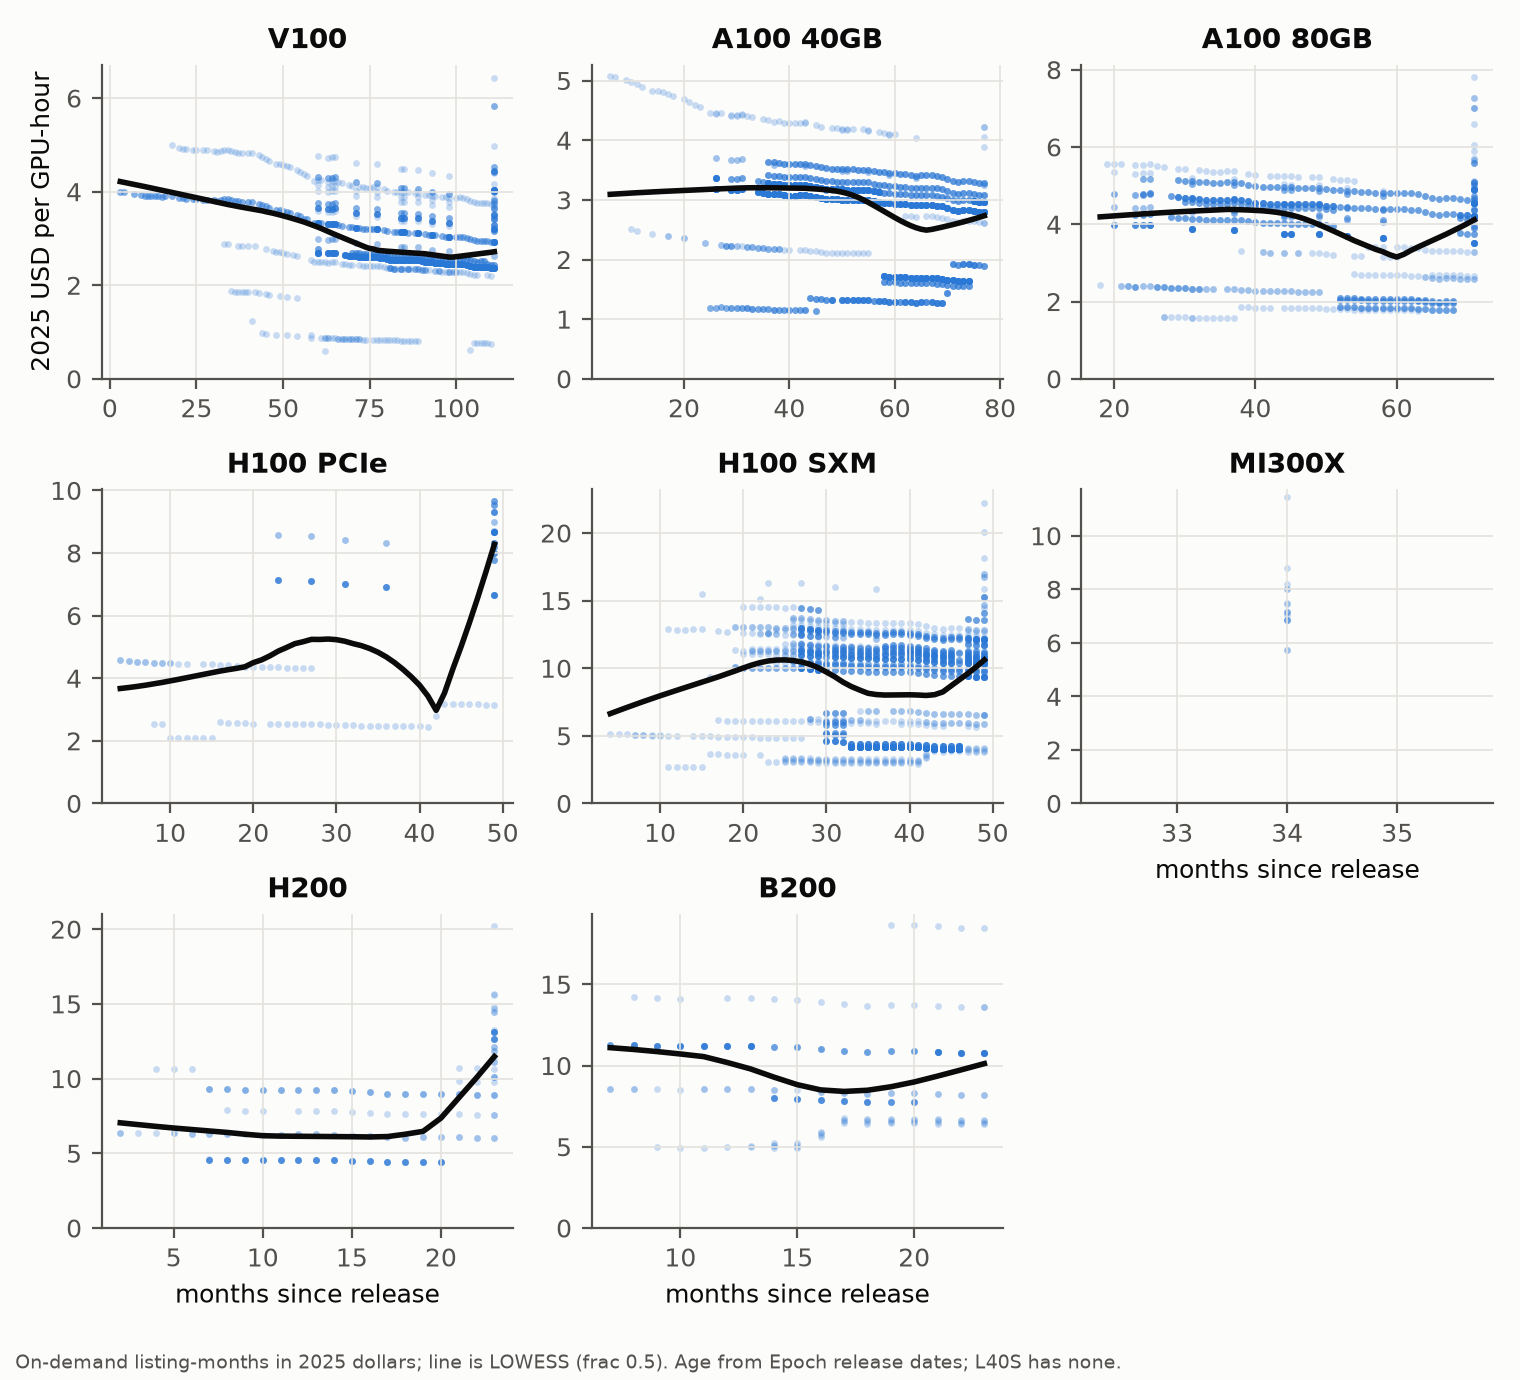
\includegraphics[width=0.49\textwidth]{p4b_price_vs_age.png}
\caption{On-demand prices by chip over time (left) and real prices against age (right). Source:
the panel described in Section~\ref{sec:data}; outlier-flagged listings excluded.}
\label{fig:prices}
\end{figure}
